\makeatletter
\def\input@path{{../../template/}}
\makeatother

\documentclass{LnxClase}

\usepackage{Lnx} % Paquete Lnx
\usepackage{LnxPost}
\usepackage{enumitem} % Paquete para personalizar listas
\usepackage{multicol}
\usepackage{graphicx}
\usepackage{pstricks} % usar \red \blue etc
\usepackage{soul} % resaltar
\usepackage{makeidx} 

\SetLnxLogo{img/logo_dark_edit.png} % cambiar el logo

\begin{document} 
	
	\SetLnxColors{LnxblackF}{white}   % fondo y tex color default
	\SetLnxRptaColors{LnxblackZ}{LnxRedD} %AA % Fes original
	
	%


\LnxExam{
	\frenchspacing
	\begin{flushleft}
		\begin{minipage}{2.3cm}
			\begin{center}
				
\includegraphics[width=0.9\linewidth]{img/logo_uni.png}
			\end{center}
		\end{minipage}
		\begin{minipage}{11cm}
			\begin{flushleft}
				{
					\Large \textsc{{\bf UNIVERSIDAD NACIONAL DE INGENIERÍA}	}		\\
					\mbox{{\bf Facultad de Ingeniería Mecánica}} \\
				}
			\end{flushleft}
		\end{minipage}
		\begin{minipage}{2.3cm} 			
			%\LnxSize{1} % Logo escalado
			
\includegraphics[width=1\linewidth]{img/logo_light_edit.png}
		\end{minipage}
	\end{flushleft}
	%%FIN
	
	\vspace{15pt}
	\begin{center}
		{\bf {\Large Segunda práctica calificada Cálculo Integral (BMA02) }}\\\vspace{.5 cm}
		{\bf {\large 2019-II}}
	\end{center}
	%fin del logo
	
	%enumeracion
	Tiempo: 3 días 
	\begin{enumerate} \item 
		{\bf Hallar los siguientes límites}
		\vspace{10pt}
		
			a) 
			$
			\displaystyle \lim_{n \rightarrow \infty } \frac{\sqrt[n]{\pqty{1^2+n^2}(2^2+n^2)\ldots ((2n)^2+n^2))}}{n^4}
			$
			\\
			b)
			$
			\displaystyle \lim_{x \rightarrow 0^{+} } \int_0^1 \frac{\ln ( x^{x^2}\sen(x \sqrt{t})+x^{x^2} )}{x}\, \mathrm{d}t
			$
		\item 
		{\bf Sea $f: \mathbb{R} \rightarrow \mathbb{R} $ una función continua. Mostrar } %Descriptor personalizado 
		\vspace{10pt}
		
		a) 
		$
		\displaystyle \int_{1}^{3} \cos (x^2-4x)(x+f(\sen (x^2-4x))(x-2)-2)=0
		$
		\\
		
		b)
		$
		\displaystyle \int_{0}^{\pi} \frac{sen(x)f(x)}{f(x)+f(\pi-x)}=1
		$
		
		\vspace{10pt}
		
		\item %problema 3
		{\bf Dado  $n \in \mathbb{N} $, a y b números positivos, hallar los siguientes integrales  } 
		\vspace{10pt}
		\begin{multicols}{2}
			
			a) 
			$
			\displaystyle \int_{0}^{\pi} \frac{x \sen^{2n+2}x \cos^2 x }{  \sen^{2n}x +\cos^{2n}x} \mathrm{d} x
			$
			\\
			b)
			$
			\displaystyle \int_{0}^{ \arctan(\frac{a}{b}) } \frac{b\sen x +a\cos x}{a\sen x+b\cos x} \, \mathrm{d} x  
			$
		\end{multicols} % Final del primer problema
		\item %problema 4
		{\bf Sea $k \in \mathbb{R } \hspace{.25 cm}\mbox{y} \hspace{.25cm} f: \mathbb{R} \rightarrow \mathbb{R} $ definidas respectivamente como}
		
		\begin{center}
			$f(x):=\displaystyle \int_{0}^{ x } e^{t^2} \, \mathrm{d}t $ , \hspace{1 cm} $k:=f(1) $
		\end{center}
		{\bf Hallar las siguientes integrales en términos de k}
		\begin{multicols}{2}
			a) 
			$
			\displaystyle \int_{0}^{ k } \left[ \frac{y}{e^{(f^{-1} (y))^2}} -f^{-1} (y) \right]\, \mathrm{d} y
			$
			\\
			b)
			$
			\displaystyle \int_{0}^{ 1 } \int_{0}^{ z } \int_{0}^{ y }  ze^{x^2+y^2}  \mathrm{d} x \  \mathrm{d} y \  \mathrm{d} z
			$
		\end{multicols} % Final del primer problema
		
	\end{enumerate}
	
} 

\newpage
\SetLnxColors{LnxblackF}{white}
\LnxSolucion{Solución}{

\solucion{Solución 1.a} 

Reescribiendo el límite,

$$
\Omega= \lim_{n \to \infty } \frac{\sqrt[n]{ \prod_{i = 1 }^{2n} (i^2 + n^2) }}{n^4} 
$$

Tomando el logaritmo natural en ambos lados,

$$
\ln (\Omega)= \lim_{n \to \infty } \ln \pqty{\prod_{ i =1 }^{2n} (i^2 + n^2)}^{1/n}-2\ln(n^2)  
$$

Se sabe que $   \ln (b)^a=a\ln(b)$

$$
\ln (\Omega)= \lim_{n \to \infty } \frac{\ln \left(    \prod_{ i =1 }^{2n} (i^2 + n^2)     \right)-2n\ln(n^2)}{n}  
$$

Además, por propiedad $ \ln(\prod_{i=1}^{n}a_i)=\sum_{i=1}^{n}\ln(a_i)$

$$
\ln (\Omega)= \lim_{n \to \infty } \frac{\pqty{\sum_{ i =1 }^{2n} \ln(i^2 + n^2)}- \sum_{i=1}^{2n}\ln(n^2)}{n}  
$$

También, $ \sum_{i=1}^{k} y_i-z_i = \sum_{i=1}^{k}y_i - \sum_{i=1}^{k} z_i $ 

$$
\ln (\Omega)=  \lim_{n \to \infty } \frac{     \sum_{ i =1 }^{2n} \left[ \ln(i^2 + n^2)   -  \ln(n^2)\right]  }{n} 
$$


$$
 \ln (\Omega) =
  \lim_{n \to \infty } \sum_{i=1}^{2n} \ln\left( \frac{i^2+n^2}{n   ^2}\right) \frac{1}{n}
$$

$$
\ln (\Omega)=  \lim_{n \to \infty }  \sum_{ i =1 }^{2n} \ln\left( \left( \frac{i}{n} \right) ^2+1\right)    \frac{1}{n} 
$$

Mediante sustitución $2n=p$

$$
\ln (\Omega)= \lim_{p \to \infty }  2\sum_{ i =1 }^{p} \ln\left( 4\left( \frac{i}{p} \right) ^2+1\right)   \frac{1}{p}
$$

\begin{definicion}
	La \textbf{integral definida de Riemann} de una función \( f(x) \) en \([a,b]\) se define como el límite de la suma de Riemann:
	\[
	\int_a^b f(x) \,dx = \lim_{n \to \infty} \sum_{i=1}^{n} f(x_i^*) \Delta x,
	\]
	donde \( x_i^* \) es un punto dentro de cada subintervalo y \( \Delta x = \frac{b-a}{n} \).
\end{definicion}

En consecuencia, tenemos

$$
\ln (\Omega) =
2\ \int_0^1 \ln(4x^2+1)\dd{x}
$$

Resolviendo la integral

$$
\ln (\Omega)=  \eval{ 2x\ln(4x^2+1)-4x+2\tan^{-1}(2x)}_0^1 
$$

$$
\ln (\Omega)= 2\ln(5)+2\arctan(2)-4 $$

\begin{LnxRptaBox}
	$$
 \Omega=25   e^{2\arctan(2)-4}
	$$
\end{LnxRptaBox}

\solucion{Solución 1.b} 

Se debe encontrar:


$$
\omega = \lim_{x \to 0^{+} }\pqty{ \int_0^1 \frac{\ln ( x^{x^2}\sen(x \sqrt{t})+x^{x^2} )}{x} \dd{t}}
$$

$$
\omega = \lim_{x \to 0^{+} } \int_0^1 x\ln (x) \dd{t}+\int_0^1 \frac{\ln ( \sen(x \sqrt{t})+1 )}{x} \dd{t}
$$

$$ 
\omega = \lim_{x \to 0^{+} } \pqty{x\ln (x)+\int_0^1 \frac{\ln ( \sen(x \sqrt{t})+1 )}{x} \dd{t}}
$$

Aplicamos la regla de L’Hôpital 

$$
\omega = \lim_{x \to  0^{+} } \pqty{ \frac{\dv{x}(\ln(x))}{\dv{x}(1/x)}+\int_0^1 \frac{\pdv{x}\ln ( \sen(x \sqrt{t})+1 )}{\pdv{x}x} \dd{t}}
$$

Observamos que operando obtenemos,

$$
\omega = \lim_{x \to 0^{+}} \pqty{-x +\int_0^1 \frac{\sqrt{t} \cos (x\sqrt{t}) }{\sen (x\sqrt{t}) +1}\dd{t}} 
$$

Mediante el límite y operando la integral
$$
\omega = \int_0^1 \sqrt{t} \dd{t}= \frac{2}{3}
$$



\begin{LnxRptaBox}
	$$
	\lim_{x \to 0^{+} }\pqty{ \int_0^1 \frac{\ln ( x^{x^2}\sen(x \sqrt{t})+x^{x^2} )}{x} \dd{t}} = \frac{2}{3}
	$$
\end{LnxRptaBox}


\solucion{Solución 2.a} 

Dada la integral

$$
 \int_1^3 \cos(x^2-4x)(x+f(\sen(x^2-4x))(x-2)-2)  
$$
 
Realizando un cambio de variable $ x-2=u$,

$$
 \int_{-1}^1 u\ \cos(u^2-4)(1+f(\sen(u^2-4)) 
$$

$$
g(u)=u\ \cos(u^2-4)(1+f(\sen(u^2-4)) 
$$
 $$
 g(-u)=-u\ \cos(u^2-4)(1+f(\sen(u^2-4)) 
 $$
 Vemos que  $g(u)$ es impar,
 
 $$
 g(u)=-g(u)
 $$
 
 \begin{proposicion}
 	Si \( g: [-b,b] \to \mathbb{R} \) es una función impar, entonces se cumple que:
 	\[
 	\int_{-b}^{b} g(u) \,du = 0.
 	\]
 \end{proposicion}
 
 Por la proposición
\begin{LnxRptaBox}
	$$
	 \int_{-1}^1 u\ \cos(u^2-4)(1+f(\sen(u^2-4)) = 0 
	$$
\end{LnxRptaBox}

\solucion{Solución 2.b} 

\begin{equation}
I=  \int_{0}^{\pi} \frac{sen(x)f(x)}{f(x)+f(\pi-x)}	
\label{eq:fim_19_2_1}
\end{equation}

Usamos la siguiente proposición,
\begin{proposicion}
	Sea \( g: [0,a] \to \mathbb{R} \) una función integrable en \([0,a]\). Entonces, se cumple la siguiente propiedad de simetría,
	\[
	\int_0^a g(x) \,dx = \int_0^a g(a-x) \,dx.
	\]
\end{proposicion}

Por lo tanto,

$$
I=  \int_{0}^{\pi} \frac{sen(\pi-x)f(\pi-x)}{f(\pi-x)+f(\pi-(\pi-x))}
$$

Simplificando  $I$,

\begin{equation}
I=  \int_{0}^{\pi} \frac{sen(x)f(\pi-x)}{f(\pi-x)+f(x)}
\label{eq:fim_19_2_2}
\end{equation}

Sumando las ecuaciones (\ref{eq:fim_19_2_1}) y  (\ref{eq:fim_19_2_2}) se tiene,

$$
2I=  \int_{0}^{\pi} \frac{sen(x)\pqty{f(x)+f(\pi-x)} }{f(x)+f(\pi-x)}
$$

Simplificando
$$
2I=  \int_{0}^{\pi} sen(x)=2
$$

\begin{LnxRptaBox}
	$$
	I= \int_{0}^{\pi} \frac{sen(x)f(x)}{f(x)+f(\pi-x)}	=  1
	$$
\end{LnxRptaBox}

\solucion{Solución 3.a} 
\begin{equation}
	I=  \int_{0}^{\pi} \frac{x \sen^{2n+2}(x) \cos^2 (x) }{  \sen^{2n}(x) +\cos^{2n}(x)} \dd{x}
	\label{eq:fim_19_2_3}
\end{equation}

De la proposición 2, tenemos

$$
I=  \int_{0}^{\pi} \frac{(\pi-x) \sen^{2n+2}(\pi-x) \cos^2 (\pi-x) }{  \sen^{2n}(\pi-x) +\cos^{2n}(\pi-x)} \dd{x}
$$

Simplificando,

\begin{equation}
	I=  \int_{0}^{\pi} \frac{(\pi-x) \sen^{2n+2}(x) \cos^2 (x) }{  \sen^{2n}(x) +\cos^{2n}(x)}\dd{x}
	\label{eq:fim_19_2_4}
\end{equation}

Sumando las ecuaciones (\ref{eq:fim_19_2_3}) y  (\ref{eq:fim_19_2_4}) se tiene,

$$
2I=  \int_{0}^{\pi} \frac{\pi \sen^{2n+2}(x) \cos^2 (x) }{  \sen^{2n}(x) +\cos^{2n}(x)} \dd{x}
$$

$$
2I= \int_{-\frac{\pi}{2}}^{\frac{\pi}{2}} \frac{\pi \cos^{2n+2}(x) \sen^2(x)}{\sen^{2n}(x)+\cos^{2n}(x)} \dd{x}
$$
\begin{proposicion}
	Si \( f: [-a,a] \to \mathbb{R} \) es una función par,  entonces se cumple la siguiente propiedad,
	\[
	\int_{-a}^{a} f(x) \,dx = 2 \int_{0}^{a} f(x) \,dx.
	\]
\end{proposicion}

De la proposición, tenemos que,

$$
 2I=   2\int_{0}^{\frac{\pi}{2}} \frac{\pi \cos^{2n+2}x \sen^2 x }{  \sen^{2n}x +\cos^{2n}x} \dd{x}
$$

\begin{equation}
	I=  \int_{0}^{\frac{\pi}{2}} \frac{\pi \cos^{2n+2}x \sen^2 x }{  \sen^{2n}x +\cos^{2n}x} \dd{x}
	\label{eq:fim_19_2_5}
\end{equation}

Usamos la primera proposición y simplificando


\begin{equation}
	I=  \int_{0}^{\frac{\pi}{2}} \frac{\pi \sen^{2n+2}x \cos^2 x }{  \sen^{2n}x +\cos^{2n}x} \dd{x
	}
	\label{eq:fim_19_2_6}
\end{equation}

Sumando las ecuaciones (\ref{eq:fim_19_2_5}) y  (\ref{eq:fim_19_2_6}) se tiene,

$$
2I=  \int_{0}^{\pi/2} \pi \sen^2 x \cos^2 x  \dd{x}  
$$

Resolviendo la integral se obtiene

$$
I=\frac{\pi^2}{32}
$$
 
\begin{LnxRptaBox}
	$$
 \int_{0}^{\pi} \frac{x \sen^{2n+2}(x) \cos^2 (x) }{  \sen^{2n}(x) +\cos^{2n}(x)} \dd{x}= \frac{\pi^2}{32}
	$$
\end{LnxRptaBox}

\solucion{Solución 3.b} 


$$
I= \int_{0}^{ \arctan(a/b) } \frac{b\sen x +a\cos x}{a\sen x+b\cos x} 
\dd{x}
$$

Dividimos entre $b$ el numerador y denominador

$$
I = \int_{0}^{ \arctan(a/b) } \frac{\sen x +\frac{a}{b}\cos x}{\frac{a}{b} \sen x+\cos x} \dd{x}   
$$

Hacemos sustitución $\frac{a}{b} =u $, entonces

$$
I= \int_{0}^{ \arctan(u) } \frac{\sen x +u\cos x}{u \sen x+\cos x}\dd{x}
$$

dividimos entre $\sen(x)$ el numerador y denominador

$$
I= \int_{0}^{ \arctan(u) } \frac{\tan x +u}{u \tan x+1} \dd{x}
$$

Usando sustitución $\tan(x) =m  \Rightarrow \dd{x} =\frac{\dd{m}}{m^2 +1} $
  
$$
 I= \ \int_{0}^{ u } \frac{m +u}{(um +1)(1+m ^2 )}\dd{m}
$$

Mediante fracciones parciales integramos
\[
\frac{m + u}{(u m + 1)(1 + m^2)} = \frac{\frac{u^3 - u}{u^2 + 1}}{u m + 1} + \frac{\frac{1 - u^2}{u^2 + 1} \cdot m}{m^2 + 1}+ \frac{\frac{2u}{u^2 + 1}}{m^2 + 1} 
\]

Entonces separamos en 3 integrales $I_1, I_2, I_3$

$
I= I_1+I_2+I_3
$ 

La primera integral $I_1$  es,

$$
I_1= \ \int_{0}^{ u } \left(\frac{u^2-1}{u^2+1} \right) \left(\frac{u}{mu+1} \right)  \, \mathrm{d} m 
$$

$$
I_1=\eval{ \left(\frac{u^2-1}{u^2+1} \right) \ln \vert um+1 \vert }_0^u = \left(\frac{u^2-1}{u^2+1} \right) \ln (u^2+1)
$$

La segunda integral $I_2$  es,

$$
I_2=\ \int_{0}^{ u }
\left( \frac{1-u^2}{2u^2+2}\right)\left(\frac{2m}{m^2+1} \right) \dd{m}
$$

$$
I_2 =\eval{ \frac{1-u^2}{2(u^2+1)} \ln (m^2+1)}_{0}^{u} = \frac{1-u^2}{2(u^2+1)} \ln (u^2+1)
$$
 
La tercera integral $I_3$  es,
 
$$
I_3= \int_{0}^{ u } \pqty{\frac{2u}{u^2+1}} \frac{1}{(m^2+1)} \dd{m}
$$

$$
I_3=\pqty{\frac{2u}{u^2+1}}\arctan(m)  \bigg \rvert_0^u=\frac{2u}{u^2+1} \arctan(u) 
$$

Sumando $\mathrm{I_1}+ \mathrm{I_2}+ \mathrm{I_3}=I$

$$
I= \frac{(u^2-1)}{2(u^2+1)} \ln (u^2+1)+\frac{2u}{u^2+1} \arctan(u)$$

donde $  u=\frac{a}{b} $, por lo tanto

\begin{LnxRptaBox}
	$$ 
	I= \frac{(a^2-b^2)}{2(a^2+b^2)} \ln \left(\frac{a^2+b^2}{b^2} \right)+\frac{2ab}{a^2+b^2} \arctan(\frac{a}{b})
	$$
\end{LnxRptaBox}

%%%%%%%%%%%%%%%%%%%%%%%%%%%%%%%%%%%%%%%%%%
\solucion{Solución 4} 

$$
f(x)=\ \int_{0}^{ x } e^{t^2} \, \mathrm{d}t \Rightarrow f(0)=0
$$

$$
f(1)=k=\ \int_{0}^{ 1 } e^{t^2}\dd{t}
$$

$$
f^{'}(x)=e^{x^2} 
$$


\solucion{Solución 4.a} 

$$ 
\mathrm{Int}= \ \int_{0}^{ k } \left[ \frac{y}{e^{(f^{-1} (y))^2}} -f^{-1} (y) \right]\, \mathrm{d} y   
$$

$$
f(f^{-1} (y))=\ \int_{0}^{ f^{-1} (y) } e^{t^2} \, \mathrm{d}t =y
$$

Tomando la primera derivada respecto a $y$, se tiene

$$
1=e^{(f^{-1} (y))^2} \left(f^{-1} (y) \right)^{'}  
\Rightarrow \frac{y}{e^{(f^{-1} (y))^2}} =y \left(f^{-1} (y) \right)^{'}
$$

$$
\mathrm{Int}= \ \int_{0}^{ k } \left[ y \left(f^{-1} (y) \right)^{'} -f^{-1} (y) \right]\, \mathrm{d} y  \hspace{.3 cm}  \hspace{.3 cm} 
$$

Hacemos sustitución $ m=f^{-1} (y)$ para continuar

$$
f^{'} (m) \, \mathrm{d} m= \mathrm{d}y \hspace{.3 cm};  \hspace{.3 cm} y=k \Rightarrow m=1 \hspace{.3 cm};  \hspace{.3 cm} y=0 \Rightarrow m=0
$$

$$
\mathrm{Int}= \ \int_{0}^{ 1 } \left[ f(m) \left(m \right)^{'} -m \right] f^{'} (m) \, \mathrm{d} m
$$

$$
\mathrm{Int}= \ \int_{0}^{ 1 }  f(m) f^{'} (m) \, \mathrm{d} m -\int_{0}^{ 1 } m e^{m^2} \, \mathrm{d} m 
$$

$$
\mathrm{Int}= \frac{f^2 (m)}{2} -\frac{e^{m^2}}{2} \bigg\rvert_0^1 
$$

\begin{LnxRptaBox}
$$ 
\mathrm{Int}= \frac{k^2 -e+1}{2}
$$
\end{LnxRptaBox}

\solucion{Solución 4.b}
 
$$
I_b= \ \int_{0}^{ 1 } \int_{0}^{ z } \int_{0}^{ y }  ze^{x^2+y^2}  \mathrm{d} x \,  \mathrm{d} y \,  \mathrm{d} z 
$$

Distribuimos las variables  

$$
I_b= \ \int_{0}^{ 1 } z \int_{0}^{ z } e^{y^2} \int_{0}^{ y }  e^{x^2}  \mathrm{d} x \,  \mathrm{d} y \, \mathrm{d} z     
$$

$$
\mathrm{I_b}= \ \int_{0}^{ 1 } z \int_{0}^{ z } e^{y^2} f(y) \,  \mathrm{d} y \,  \mathrm{d} z  =\int_0^1 z \int_0^z f^{'}(y)f(y)\, \mathrm{d} y \, \mathrm{d } z     
$$

$$ 
\mathrm{I_b}= \ \int_{0}^{ 1 } z \left[ \frac{f^2(y)}{2} \bigg \rvert_0^z \right]  \,  \mathrm{d} z  =\frac{1}{2}\int_0^1 z f^2(z)  \, \mathrm{d } z     
$$


Integramos por partes  $\displaystyle \int zf^2(z) \, \mathrm{d} z$
 \begin{itemize}
 	\item[] $z\, \mathrm{d} z=\mathrm{d} v\Rightarrow \frac{z^2}{2}=v$
 	\item[] $ f^2(z)=u \Rightarrow 2f^{'}(z) f(z) \, \mathrm{d} z =\mathrm{d}u$
 \end{itemize}

Reemplazando en $\int u \dd{v}=uv-\int v \dd{u}$
$$
2I_b= \int zf^2(z) \, \mathrm{d} z=\frac{z^2 f^2(z)}{2}- \int z^2 f^{'}(z) f(z) \, \mathrm{d} z 
$$

$$
2I_b=\ \int zf^2(z) \, \mathrm{d} z=\frac{z^2 f^2(z)}{2}- \int z f(z) z e^{z^2}  \, \mathrm{d} z 
$$ 

Integramos por partes, $\displaystyle I_c= \int z f(z) z e^{z^2} \, \mathrm{d} z$

 \begin{itemize}
	\item[] $z e^{z^2}\, \mathrm{d} z=\mathrm{d} m\Rightarrow \frac{ e^{z^2}}{2}=m$
	\item[] $zf(z)=n \Rightarrow (f(z)+zf^{'}(z))\, \mathrm{d} z =\mathrm{d}n$
\end{itemize}
 
$$
I_c=\ \int z f(z) z e^{z^2} \, \mathrm{d} z=\frac{ze^{z^2}f(z)}{2}-\int \frac{e^{z^2}}{2} \left(f(z)+zf^{'}(z) \right) \, \mathrm{d} z 
$$

$$
I_c=\frac{ze^{z^2}f(z)}{2}-\int \frac{f^{'}(z)f(z)}{2} \, \mathrm{d} z -\frac{1}{2} \int z e^{2z^2}  \, \mathrm{d} z 
$$

$$
I_c=\frac{ze^{z^2}f(z)}{2}- \frac{f^2(z)}{4}  -\frac{1}{8}  e^{2z^2} +C
$$

Reemplazando en $2I_b$

$$
\ \int zf^2(z) \, \mathrm{d} z=\frac{z^2 f^2(z)}{2}- \frac{ze^{z^2}f(z)}{2}+ \frac{f^2(z)}{4}  +\frac{1}{8}  e^{2z^2} +C
$$

$$ 
\mathrm{I_b}= \frac{1}{2}\int_0^1 z f^2(z)  \, \mathrm{d } z  =   
$$

$$ 
\mathrm{I_b}=   \frac{(2z^2+1) f^2(z)}{8}- \frac{ze^{z^2}f(z)}{4}  +\frac{1}{16} e^{2z^2} 
\bigg \rvert_0^1 
$$

Por lo tanto, tenemos

\begin{LnxRptaBox}
$$ 
\mathrm{I_b}=\frac{3k^2-2ek}{8}+\frac{e^2-1}{16}
$$
\end{LnxRptaBox}


}
 % falta ordenar
	 
	%Ley de Exponentes
\vspace{-5cm}
\LnxPregunta{ \quad Ley de exponentes  }{
	\centering
	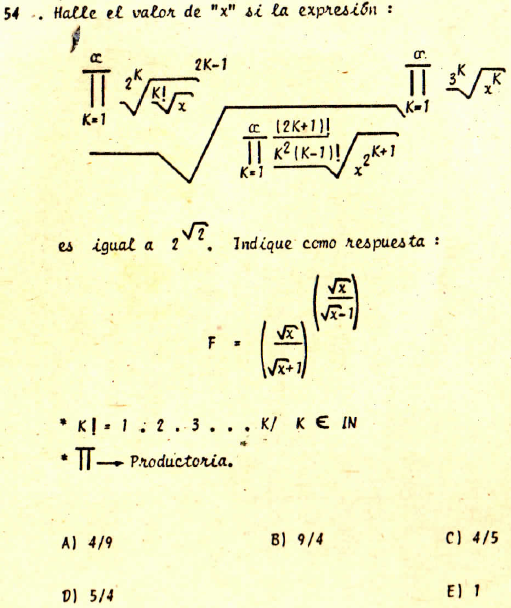
\includegraphics[width=0.95\linewidth]{algebra_pre/Pro_001.png}
}

\LnxSolucion{Solución}{
Sea
$$
	\sqrt[\beta]{\theta}^{\alpha} = 2^{\sqrt{2}}
$$
donde $\alpha, \beta$ y $\theta$ son:
\begin{equation*}
	\scalebox{0.95}{$\displaystyle
			\alpha=\prod_{k= 1}^{\infty} \sqrt[3^k]{x^k}, \quad  \beta = \prod_{k=1}^\infty \left( \sqrt[2^k]{ \sqrt[k!]{x} } \right)^{2k - 1}, \quad \theta = \prod_{k=1}^\infty  \sqrt[\frac{(2k+1)!}{k^2 \cdot (k-1)!} \;\;\; ]{ \displaystyle x^{2^{k+1}}}
		$}
\end{equation*}
Calculamos $\alpha$, [{\small(La demostración de la convergencia queda como ejercicio para el lector)}]
$$
	\alpha=\prod_{k= 1}^{\infty} \sqrt[3^k]{x^k} = (x)^{\sum_{k=1}^{\infty} k\cdot 3^{-k}}
$$
Por la serie geométrica  para \(|u| < 1\),
\begin{equation*}
	\scalebox{0.8}{$\displaystyle
			\sum_{k=1}^\infty k u^k = u \bqty{\dv{u}(\sum_{k=0}^\infty u^k) } = u \bqty{\dv{u}(\frac{1}{1 - u}) }
			= \frac{u}{(1 - u)^2}
		$}
\end{equation*}
$$
	\rightarrow \alpha  =  (x)^{\sum_{k=1}^{\infty} k\cdot 3^{-k}}= (x)^{\frac{ 1/3}{(1-1/3)^2 } } = x^{3/4}
$$

Calculamos $\beta$, [{\small(La demostración de la convergencia queda como ejercicio para el lector)}]
$$
	\beta = \prod_{k=1}^\infty \left( \sqrt[2^k]{ \sqrt[k!]{x} } \right)^{2k - 1} = x ^{ \sum_{k=1}^{\infty} \frac{2k-1}{2^k \cdot k!}}
$$
Calculando  el exponente  $\sum_{k=1}^{\infty} \frac{2k - 1}{2^k \cdot k!}$,

\begin{align*}
	\sum_{k=1}^{\infty} \frac{2k - 1}{2^k \cdot k!}
	 & = \sum_{k=1}^\infty \frac{1}{2^{k-1} \cdot (k-1)!} - \sum_{k=1}^\infty \frac{1}{2^k \cdot k!} \\
	 & = \sum_{k=0}^\infty \frac{1}{2^k \cdot k!} - \sum_{k=1}^\infty \frac{1}{2^k \cdot k!}  = 1
\end{align*}
$$
	\Rightarrow \beta =x^{1}=x
$$
Calculamos $\theta$, [{\small(La demostración de la convergencia queda como ejercicio para el lector)}]
\[
	\theta = \prod_{k=1}^\infty  \sqrt[\frac{(2k+1)!}{k^2 \cdot (k-1)!} \;\;\; ]{ \displaystyle x^{2^{k+1}}}  = (x)^{\sum_{k=1}^\infty \frac{2^{k+1}\cdot k^2 \cdot (k-1)!}{ (2k+1)!}}
\]
Calculando  el exponente  $ \sum_{k=1}^\infty \frac{2^{k+1}\cdot k^2 \cdot (k-1)!}{ (2k+1)!}$,
\begin{align*}
	\sum_{k=1}^\infty \frac{2^{k+1}\cdot k  \cdot (k )!}{ (2k+1)!} & =\frac{1}{2}\bqty{   \sum_{k=1}^\infty \frac{2^{k}  \cdot (k-1 )!}{ (2k-1)!}- \frac{2^{k+1}\cdot   (k )!}{ (2k+1)!}}                      \\
	                                                               & =\frac{1}{2}\pqty{2+\sum_{k=1}^\infty \frac{2^{k+1}\cdot   (k )!}{ (2k+1)!} - \sum_{k=1}^\infty \frac{2^{k+1}\cdot   (k )!}{ (2k+1)!} }=1
\end{align*}
$$
	\rightarrow \theta = x ^1 = x
$$
Entonces, reemplazando $\alpha, \beta $ y $\theta$:
$$
	\sqrt[\beta]{\theta}^{\alpha} =\sqrt[x]{x}^{x^{3/4}} = x^{x^{-1/4}} =2^{\sqrt{2}}
$$
Elevamos a $(-1/4)$
$$
	\pqty{x^{-1/4}}^{\pqty{ x^{-1/4}}} = \pqty{2^{\sqrt{2}} }^{-1/4}= \pqty{\frac{1}{2}}^{\frac{\sqrt{2}}{4}}= \pqty{\frac{1}{\sqrt{2}}}^{\pqty{\frac{1}{\sqrt{2}}}}
$$
$$
	x^{-1/4} = \frac{1}{\sqrt{2}} \Rightarrow x^{1/4} = \sqrt{2} \Rightarrow x = (\sqrt{2})^4 = 4
$$

Finalmente, reemplazamos $x$ en $F$,
}

\begin{LnxRptaBox}
	\[
		F= \pqty{\frac{\sqrt{x}}{\sqrt{x}+1}}^{\pqty{\frac{\sqrt{x}}{\sqrt{x}-1}}} = \pqty{\frac{2}{3}}^{\frac{2}{1}}= \frac{4}{9}
	\]
\end{LnxRptaBox}
 
\newpage
\LnxPregunta{Calcule el  limite,\\
\begin{equation*}
	\lim\limits_{x \to 0} 
	\frac{\displaystyle \int_{1}^{\infty} \frac{\ln^x(t)}{t^{2\gamma}} \dd{t}-(2\gamma-1)^{-x-1}}{e^x-1}
\end{equation*}\\
{\LARGE donde $\gamma$ es la constante de Euler-Mascheroni.}
}

\LnxSolucion{Solución}{
	
	Resolvemos la integral, hacemos $\ln(t)=u \rightarrow \frac{\dd{t}}{t}=\dd{u}$
	
	$$
	 I=\int_{1}^{\infty} \frac{\ln^x(t)}{t^{2\gamma}} \dd{t}=\int_{0}^{\infty} u^x e^{2(\gamma-1)u} \dd{u}
	$$
	
	Hacemos otro cambio de variable,	
	 $(2\gamma-1)u=v$ 
	
	\[
	I= \frac{1}{(2\gamma-1)^{x+1}} \int_{0}^{\infty} v^x
	e^{-v} \dd{v}	=\frac{\Gamma(x+1)}{(2\gamma-1)^{x+1}}
	\]
	
	Sea $L$ el límite
	
	\[
	L=\lim\limits_{x \to 0} 
	\frac{\displaystyle I-(2\gamma-1)^{-x-1}}{e^x-1}
	\]
	
	\[
	L=\lim\limits_{x \to 0} 
	\frac{\displaystyle (2\gamma-1)^{-x-1}\ \Gamma(x+1)-(2\gamma-1)^{-x-1}}{e^x-1}
	\]
	
	\[
	L=\lim\limits_{x \to 0} \frac{1}{(2\gamma-1)^{x+1}} \cdot
	\frac{\displaystyle  \Gamma(x+1)-1}{e^x-1}
	\]
	
	Sabemos que 
	
		\[
	\lim\limits_{x \to 0}
	\frac{e^x-1}{x}=1
	\]
	
		\[
	\lim\limits_{x \to 0}
	\frac{\Gamma(x+1)-1}{x}=\Gamma^{'}(1)=-\gamma
	\]
	
}

Reemplazando los límites en L
$$
	L=\lim\limits_{x \to 0} \frac{1}{(2\gamma-1)^{x+1}} \cdot
\frac{\displaystyle \frac{ \Gamma(x+1)-1}{x}}{\displaystyle\frac{{e^x-1}}{x}}
$$

	$$
L= \frac{1}{(2\gamma-1)} \cdot
\frac{-\gamma}{1}
$$

Entonces el valor del límite es,

\begin{LnxRptaBox}
	$$
	 \lim\limits_{x \to 0} 
	 \frac{\displaystyle \int_{1}^{\infty} \frac{\ln^x(t)}{t^{2\gamma}} \dd{t}-(2\gamma-1)^{-x-1}}{e^x-1}=\frac{\gamma}{1-2\gamma} 
	$$
\end{LnxRptaBox}
 
\newpage
\LnxPregunta{Calcule el valor del límite,}{
\Huge
\begin{equation*}
	\lim_{x \to \infty} \pqty{ \frac{1}{x} \pqty{ \frac{\zeta(1 + \frac{1}{x})}{x} }^{\frac{x}{\gamma}} \ \pqty{ \frac{(2x)!}{x!} }^{\frac{1}{x}} - 4 } x
\end{equation*}
%{\Huge es}  \quad
%$
%2 \log(2) - \frac{4 \gamma_1}{\gamma} - 2 \gamma
%$
\\
{\LARGE 
\begin{itemize}[label=\textcolor{white}{$\circ$}] % Usa un círculo como viñeta
	\item $ \gamma$ es la constante de Euler-Mascheroni.
	\item $\gamma_1$ es la primera constante de Stieltjes.
	\item $\zeta(s) =\displaystyle \sum_{n=1}^{\infty} \frac{1}{n^s}$ es la función zeta de Riemann.
\end{itemize}
}
}

\LnxSolucion{Solución}{
Definimos la expresión y calculamos su aproximación,

\[
A = \left( \frac{\zeta(1 + \frac{1}{x})}{x} \right)^{\frac{x}{\gamma}}
\]

Mediante la expansión de Laurent para $s=1$, tenemos que

\[
\zeta(s) \approx \frac{1}{s-1} + \gamma + \sum_{k=1}^{\infty} \frac{(-1)^k \gamma_k}{k!} (s-1)^k
\]

Sustituyendo $s = 1 + \frac{1}{x}$,

\[
\zeta\left(1 + \frac{1}{x}\right) \approx x + \gamma + \sum_{k=1}^{\infty} \frac{(-1)^k \gamma_k}{k!} \left( \frac{1}{x} \right)^k
\]

Dividiendo entre $x$,

\[
\frac{\zeta(1 + \frac{1}{x})}{x} \approx 1 + \frac{\gamma}{x} -\frac{\gamma_1}{x^2} + \mathcal{O}\left(\frac{1}{x^3}\right)
\]

Aproximamos ahora $A$ usando logaritmos,

\[
\ln A = \frac{x}{\gamma} \ln \left( \frac{\zeta(1 + \frac{1}{x})}{x} \right)
\]

Usando  $\ln(1 + a) \approx a - \frac{a^2}{2} + \mathcal{O}(a^3)$

\[
\ln A \approx \frac{x}{\gamma} \left( \frac{\gamma}{x} - \frac{\gamma_1}{x^2} - \frac{\gamma^2}{2x^2} + \mathcal{O}\left(\frac{1}{x^3}\right) \right)
\]

Multiplicando por $\frac{x}{\gamma}$,

\[
\ln A \approx 1 - \frac{\gamma_1}{\gamma x} - \frac{\gamma}{2x} + \mathcal{O}\left(\frac{1}{x^2}\right)
\]

Sea $a$ muy pequeño y $e^a=1+a+\frac{a^2}{2}+\cdots$,
$$
e^{1+a}=e^{1}\cdot e^a \approx e\pqty{1+a}+\mathcal{O}\left(a^2\right)
$$
Entonces, tomando la exponencial,
\[
A = e^{1 - \frac{\gamma_1}{\gamma x} - \frac{\gamma}{2x} + \mathcal{O}\left(\frac{1}{x^2}\right)} \approx e \left(1 - \frac{\gamma_1}{\gamma x} - \frac{\gamma}{2x} \right) + \mathcal{O}\left(\frac{1}{x^2}\right)
\]
Definimos la expresión y calculamos su aproximación,
\[
B = \left( \frac{(2x)!}{x!} \right)^{\frac{1}{x}}
\]

Usando la aproximación de Stirling $n! \approx \sqrt{2\pi n} \left(\frac{n}{e}\right)^n$, 
\[
\frac{(2x)!}{x!} \approx \frac{(2x)^{2x} e^{-2x} \sqrt{4\pi x}}{x^x e^{-x} \sqrt{2\pi x}} = 2^{2x} x^x e^{-x} \sqrt{2}
\]

Distribuyendo la potencia

\[
B = \left( \frac{(2x)!}{x!} \right)^{\frac{1}{x}} \approx 4 x e^{-1} \sqrt[2x]{2}.
\]

Usando $2^{1/2n} =e^{\ln(2)/2n}\approx 1 + \frac{\ln(2)}{2n}$,

\[
B \approx 4 x e^{-1} \left(1 + \frac{\ln(2)}{2x}\right) + \mathcal{O}\left(\frac{1}{x}\right)
\]

Multiplicamos las aproximaciones de $A$ y $B$:

\[
A \cdot B = 4 \left(x - \frac{\gamma_1}{\gamma} - \frac{\gamma}{2} + \frac{\ln(2)}{2}\right) + \mathcal{O}\left(\frac{1}{x}\right)
\]

Finalmente, calculamos el límite:
\[
L=\lim_{x \to \infty} \left(\frac{1}{x} A \cdot B - 4 \right)x = \lim_{x \to \infty} \left(A \cdot B - 4x \right)
\]
Sustituyendo la expresión obtenida:
\[
L=\lim_{x \to \infty} \left(4x + 2 \ln(2) - \frac{4 \gamma_1}{\gamma} - 2 \gamma - 4x + \mathcal{O}\left(\frac{1}{x}\right) \right)
\]
Simplificando,
\[
L=\lim_{x \to \infty} \left( 2 \ln(2) - \frac{4 \gamma_1}{\gamma} - 2 \gamma +\mathcal{O}\left(\frac{1}{x}\right)\right)
\]
}

Finalmente, tenemos que el valor del límite es
\begin{LnxRptaBox}
	\[
	L=  2\ln(2)- \frac{4 \gamma_1}{\gamma} - 2 \gamma
	\]
\end{LnxRptaBox}

\vspace{1.4cm}
{\large   * Considerar que $a$ es muy pequeño para $\ln(1+a), e^{1+a}$ y $n$ muy grande para $ n!, 2^{1/2n}$}

\newpage
\LnxPregunta{Evalúe el siguiente límite,}{
	\begin{equation*}
		\lim_{n \to \infty} \left( \begin{array}{cc} 1 &\quad \displaystyle\frac{\alpha}{n} \\ -\displaystyle\frac{\alpha}{n} & \quad 1 \end{array} \right)^n
	\end{equation*}
}

\LnxSolucion{Solución}{
	La matriz

	$$
		\left( \begin{array}{cc} 1 & \frac{\alpha}{n} \\ -\frac{\alpha}{n} & 1 \end{array} \right)
	$$
	Podemos reescribir  como,
	\begin{equation*}
		I + \frac{A}{n}, \quad \text{donde } A = \begin{pmatrix} 0 & \alpha \\ -\alpha & 0 \end{pmatrix}
	\end{equation*}

	Se puede verificar que,
	\begin{equation*}
		A = -\alpha \begin{pmatrix} \cos\left(\frac{\pi}{2}\right) & -\sin\left(\frac{\pi}{2}\right) \\ \sin\left(\frac{\pi}{2}\right) & \cos\left(\frac{\pi}{2}\right) \end{pmatrix}
	\end{equation*}

	Para una potencia $k$ de $A$,
	\begin{equation*}
		A^k = (-\alpha)^k \begin{pmatrix} \cos\left(\frac{k\pi}{2}\right) & -\sin\left(\frac{k\pi}{2}\right) \\ \sin\left(\frac{k\pi}{2}\right) & \cos\left(\frac{k\pi}{2}\right) \end{pmatrix}
	\end{equation*}

	Aplicamos la exponencial de matrices,
	\begin{equation*}
		\lim_{n \to \infty} \left( I + \frac{A}{n} \right)^n = e^A = \sum_{k=0}^{\infty} \frac{A^k}{k!}
	\end{equation*}

	Expandiendo la serie,
	\begin{equation*}
		\sum_{k=0}^{\infty} \frac{(-\alpha)^k}{k!} \begin{pmatrix} \cos\left(\frac{k\pi}{2}\right) & -\sin\left(\frac{k\pi}{2}\right) \\ \sin\left(\frac{k\pi}{2}\right) & \cos\left(\frac{k\pi}{2}\right) \end{pmatrix}
	\end{equation*}

	Calculando los t\'erminos,
	\begin{align*}
		\sum_{k=0}^{\infty} \frac{(-\alpha)^k \cos\left(\frac{k\pi}{2}\right)}{k!} & = \cos(\alpha), \\
		\sum_{k=0}^{\infty} \frac{(-\alpha)^k \sin\left(\frac{k\pi}{2}\right)}{k!} & = -\sin(\alpha)
	\end{align*}

	Por lo tanto, el límite de la matriz es,

}


\begin{LnxRptaBox}
	\begin{equation*}
		\lim_{n \to \infty} \left( \begin{array}{cc} 1 & \frac{\alpha}{n} \\ -\frac{\alpha}{n} & 1 \end{array} \right)^n = \begin{pmatrix} \cos(\alpha) & \sin(\alpha) \\ -\sin(\alpha) & \cos(\alpha) \end{pmatrix}
	\end{equation*}
\end{LnxRptaBox}

\newpage
\LnxPregunta{Calcule la integral,}{
	$$
		\int_0^1 (x^x)^{(x^x)^{(x^x)^{(x^x)^{(x^x)^{\cdots}}}}} \dd{x}
	$$
}

\LnxSolucion{Solución}{

	Sea \( y = (x^x)^{(x^x)^{(x^x)^{\cdots}}} \), entonces

	$$
		y = x^{xy}
	$$

	Definimos \( y = \frac{t}{x} \),

	$$
		y = x^t, \quad x = t^{\frac{1}{1+t}}, \quad y = \frac{t}{x} = t^{\frac{t}{1+t}}
	$$

	Ahora, consideremos la integral,

	$$
		I = \int_0^1 (x^x)^{(x^x)^{(x^x)^{\cdots}}} dx = \int_0^1  y \dd{x}
	$$

	Usando el cambio de variable \( x = t^{1+t} \),

	$$
		I = \int_0^1 t^\frac{t}{1+t} \left( \frac{-\ln t}{(1+t)^2} + \frac{1}{(1+t)t} \right)t^\frac{1}{1+t} \dd{t}
	$$

	$$
		I	= \int_0^1 \left( \frac{1}{1+t} - \frac{t \ln t}{(1+t)^2} \right) dt
	$$

	$$
		I=\eval{\ln(1+t)}_{0}^{1}-\int_0^1 \frac{t \ln t}{(1+t)^2} dt
	$$

	$$
		I	= \ln(2) - \int_0^1 \frac{t \ln t}{(1+t)^2} \dd{t}$$

	$$
		I= \ln(2)-\int_{0}^{1} \int_0^t \frac{t}{(1+t)^2 u} \dd{u} \dd{t}
	$$

	$$
		I=\ln(2)+\int_0^1 \frac{1}{u} \int_{0}^{u} \frac{t}{(1+t)^2} \dd{t} \dd{u}
	$$

	$$
		I=\ln(2)+\int_0^1 \frac{1}{u} \int_{1}^{1+u} \frac{t-1}{t^2} \dd{t} \dd{u}
	$$

	$$
		I=\ln(2)+\int_0^1 \frac{1}{u}
		\pqty{\ln(1+u)+\frac{1}{1+u}-1} \dd{u}
	$$

	$$
		I=\ln(2)+\int_0^1 \frac{\ln(1+u)}{u}\dd{u} -\ln(2)
	$$



	Usando y expansión en series para $\ln(1+u)$,
	$$
		I=  \int_0^1 \frac{1}{u} \sum_{k=1}^{\infty}  \frac{(-1)^{k+1} u^k }{k} \dd{u}
	$$

	$$
		I= \sum_{k=1}^{\infty} \frac{(-1)^{k+1}}{k} \int_0^1 u^{k-1} \dd{u}
	$$

	$$
		I	= \sum_{k=1}^{\infty} \frac{(-1)^{k+1}}{k^2} = \eta(2) = \frac{\pi^2}{12}
	$$

	Finalmente, el valor de $I$ es,
}



\begin{LnxRptaBox}
	$$
		\int_0^1 (x^x)^{(x^x)^{(x^x)^{(x^x)^{(x^x)^{\cdots}}}}} \dd{x} = \frac{\pi^2}{12}
	$$
\end{LnxRptaBox}

\newpage
\LnxPregunta{Calcule el límite,}{
$$ \lim_{n\to\infty} \lim_{x\to 2} \;\frac{\overbrace{(((x!)!)! \ldots)!}^{n \; \text{veces} } -2}{\underbrace{(((x!)!)! \ldots)!}_{n-1 \; \text{veces} } -2}
$$
}

\LnxSolucion{Solución}{
Sea $f_n(x)= (((x!)!)!\;  \ldots)! \; (n\  \text{veces})$  $\to f_n(2)=2$\ y $g(x)=x!=\Gamma(x+1)$ entonces $\ g(f_n(2))=g(2)=2 $

$$
	\Omega=
	\lim_{n\to \infty} \lim_{x\to 2} \frac{g(f_{n-1}(x))-2}{f_{n-1}(x)-2}= 	\lim_{n\to \infty} \lim_{x\to 2} \frac{2-2}{2-2}= \frac{0}{0}
$$

Mediante la regla de L'Hôpital

$$
	\Omega=  	\lim_{n\to \infty} \lim_{x\to 2}  \frac{g'(f_{n-1}(x))f'_{n-1}(x)}{f'_{n-1}(x)}=	\lim_{n\to \infty} \lim_{x\to 2} g'(f_{n-1}(x))
$$

$$
	\Omega= \lim_{n\to \infty} \lim_{x\to 2} \Gamma'(f_{n-1}(x)+1)=\lim_{n\to \infty} \Gamma'(f_{n-1}(2)+1)
$$

Si $\psi$ es la función Digamma, $ \rightarrow \Gamma'(x)=\Gamma(x)\psi(x)$\\
además,  $\displaystyle\psi(n+1)=-\gamma+\sum_{k=1}^{n} \frac{1}{k} , \quad \text{para todo } n \in \mathbb{N}$

$$
	\Omega=\Gamma'(3)= \Gamma(3)\psi(3)=2\pqty{1+\frac{1}{2}-\gamma}
$$
}
\begin{LnxRptaBox}
	$$\lim_{n\to\infty} \lim_{x\to 2} \;\frac{{(((x!)!)! \ldots)!}_{(n \; \text{veces} )} -2}{{(((x!)!)! \ldots)!}_{(n-1 \; \text{veces} )} -2}=3-2\gamma $$
\end{LnxRptaBox}
Donde $\gamma$  es la constante de Euler-Mascheroni.


\newpage
\LnxPregunta{Pruebe  que,}{
	$$
		\displaystyle \int_0^1 x^2 \psi(x) \, dx = \ln\left(\dfrac{A^2}{\sqrt{2\pi}} \right)
	$$
}

\LnxSolucion{Solución}{

	Utilizando la descomposición fraccionaria parcial de $\psi(x)$,

	$$
		\psi(x) =  -\gamma +\lim_{n\to\infty} \pqty{ H_{n+1} - \frac{1}{x} - \sum_{k=1}^{n} \frac{1}{k+x} }
	$$

	Reemplazando en la integral,
	$$
		I= \lim_{n\to\infty} \int_{0}^{1} x^2 \left( -\gamma + H_{n+1} - \frac{1}{x} - \sum_{k=1}^{n} \frac{1}{k+x} \right) \dd{x}
	$$
	Integrando

	$$
		I= \lim_{n\to\infty} \int_{0}^{1} \left( \pqty{-\gamma + H_{n+1} }x^2- x - \sum_{k=1}^{n} \frac{x^2}{k+x} \right) \dd{x}
	$$

	$$
		I=\lim_{n\to\infty}  \left(  \eval{\pqty{-\gamma + H_{n+1} }\frac{x^3}{3}- \frac{x^2}{2}}_{0}^{1} - \sum_{k=1}^{n} \int_{0}^{1}\frac{x^2}{k+x} \dd{x} \right)
	$$

	Sea la integral, [Demostración para el lector]
	$$\displaystyle \int_{0}^{1}\frac{x^2}{k+x} \dd{x} = \frac{1}{2} - k + k^2 ( \ln(1 + k)-\ln(k) )
	$$
	Entonces,
	$$
		\sum_{k=1}^{n} \int_{0}^{1}\frac{x^2}{k+x} \dd{x}=\sum_{k=1}^{n} \pqty{ \frac{1}{2} - k + k^2 ( \ln(1 + k)-\ln(k) ) }
	$$

	$$
		\sum_{k=1}^{n} \int_{0}^{1}\frac{x^2}{k+x} \dd{x}=
		\frac{n}{2}-\frac{n(n+1)}{2}- \sum_{k=1}^{n} k^2 (\ln k - \ln(k+1))
	$$

	$$
		\sum_{k=1}^{n} \int_{0}^{1}\frac{x^2}{k+x} \dd{x}=
		-\frac{n^2}{2}- \sum_{k=1}^{n} k^2 (\ln k - \ln(k+1))
	$$

	%	$$
	%	\sum_{k=1}^{n} \int_{0}^{1}\frac{x^2}{k+x} \dd{x}=	-\pqty{\frac{n^2}{2}+ \sum_{k=1}^{n} (2k-1)\ln k + n^2 \ln(n+1) }
	%	$$

	Reemplazando en el límite,

	$$
		I=\lim_{n\to\infty} \left( \frac{H_{n+1}-\gamma}{3}  - \frac{1}{2}+ \frac{n^2}{2} + \sum_{k=1}^{n} k^2 (\ln k - \ln(k+1)) \right)
	$$

	$$
		I=\lim_{n\to\infty} \left( \frac{1}{3}\ln n  - \frac{1}{2} + \frac{n^2}{2}+ \sum_{k=1}^{n} (2k-1)\ln k - n^2 \ln(n+1) \right)
	$$


	Sean $(A_n)$ y $(B_n)$ denotados por,

	$$
		A_n = \frac{1^1 2^2 \cdots n^n}{n^{n^2/2+n/2+1/12}\; e^{-n^2/4}}
		\quad \text{y} \quad
		B_n = \frac{n!}{e^{-n}\; n^{n+1/2}}
	$$

	Sabemos que $A_n \rightarrow A$ y $B_n\rightarrow \sqrt{2\pi}$

	Podemos reescribir estas definiciones, mediante $\ln (.)$

	$$
		\sum_{k=1}^{n} k \ln k
		= \ln A_n + \left( \frac{n^2}{2} + \frac{n}{2} + \frac{1}{12} \right) \ln n - \frac{n^2}{4}
	$$

	$$
		\sum_{k=1}^{n} \ln k
		= \ln B_n + \left(n + \frac{1}{2}\right) \ln n - n.
	$$






	Reemplazando  $ \displaystyle \sum_{k=1}^{n} k \ln k$  \, y \,  $\displaystyle\sum_{k=1}^{n} \ln k $ en el límite

	$$
		I= \lim_{n\to\infty} \left(2\ln A_n - \ln B_n - n^2 \ln\left(1+\frac{1}{n}\right) + n - \frac{1}{2} \right)
	$$

	Tomando límite, tenemos

	$$
		I= 2\ln A - \ln\sqrt{2\pi}
	$$



}
\begin{LnxRptaBox}
	$$
		\int_0^1 x^2 \psi(x) \, dx = \ln\left(\dfrac{A^2}{\sqrt{2\pi}} \right)
	$$
\end{LnxRptaBox}
Donde $A$  es la constante de Glaisher-Kinkelin \\

\newpage
\LnxPregunta{}{ 
	\begin{flushleft}  \Huge
		Dado  $A \in \mathcal{M}_2(\mathbb{R})$ es una matriz con dos autovalores reales  $\lambda_1 \neq \lambda_2$ y $\lambda_1 \lambda_2 > 0$.\\
		Evalue la integral,
	\end{flushleft}
	\vspace{1.5cm}
	$$
		I = \int_0^\infty \frac{\sin(Ax)}{x} dx
	$$
}

\LnxSolucion{Solución}{ 

Como $A$ es diagonalizable,

$$
A = P J_A P^{-1}, \quad \text{donde} \quad J_A = \begin{pmatrix} \lambda_1 & 0 \\ 0 & \lambda_2 \end{pmatrix}
$$

Aplicamos esta transformación a la integral,

$$
I = \int_0^\infty \frac{\sin(Ax)}{x} dx = P \left( \int_0^\infty \frac{\sin(J_A x)}{x} dx \right) P^{-1}
$$

Dado que $J_A$ es diagonal,

$$
\int_0^\infty \frac{\sin(J_A x)}{x} dx =
\begin{pmatrix}
\displaystyle \int_0^\infty \frac{\sin(\lambda_1 x)}{x} dx & 0 \\
0 &\displaystyle \int_0^\infty \frac{\sin(\lambda_2 x)}{x} dx
\end{pmatrix}
$$

Sabemos por Dirichlet’s integral que,

$$
\int_0^\infty \frac{\sin(\lambda x)}{x} dx = \operatorname{sign}(\lambda) \frac{\pi}{2}
$$

Por lo tanto,

$$
\int_0^\infty \frac{\sin(J_A x)}{x} dx =
\begin{pmatrix}
\operatorname{sign}(\lambda_1) \frac{\pi}{2} & 0 \\
0 & \operatorname{sign}(\lambda_2) \frac{\pi}{2}
\end{pmatrix}
$$
\newpage
Dado que $\lambda_1$ y $\lambda_2$ tienen el mismo signo,

$$
\int_0^\infty \frac{\sin(J_A x)}{x} dx =	\operatorname{sign}(\lambda_1) \frac{\pi}{2} I_2.
$$

Finalmente, aplicamos la transformación inversa,

$$
I = P \left( \operatorname{sign}(\lambda_1) \frac{\pi}{2} I_2 \right) P^{-1}
$$

$$
I = \operatorname{sign}(\lambda_1) \frac{\pi}{2}  P  I_2  P^{-1}
$$

Como la identidad conmuta con cualquier matriz,

$$
I = \operatorname{sign}(\lambda_1) \frac{\pi}{2} I_2
$$

Por lo tanto,   
}
\begin{LnxRptaBox}
	$$
	\int_0^\infty \frac{\sin(Ax)}{x} dx =
	\begin{cases}
		\frac{\pi}{2} I_2, & \text{si } \lambda_1, \lambda_2 > 0 \\
		&\\
		-\frac{\pi}{2} I_2, & \text{si } \lambda_1, \lambda_2 < 0
	\end{cases}
	$$
\end{LnxRptaBox} 

\newpage
\LnxPregunta{		Evalue la integral,}{  
	\vspace{1.5cm}
	$$
	\int_{0}^{\infty} \psi^{(2)} (1+x) \ln (x) \dd{x} 
	$$
	\vspace{0.1cm}
		\begin{flushleft}
		{\Huge donde $\psi$ es la función polygamma }
	\end{flushleft}
}

\LnxSolucion{Solución}{ 

Usamos la identidad de la función poligamma de orden 2,

$$
\psi^{(2)}(x) = -2 \sum_{n=0}^{\infty} \frac{1}{(n+x)^3}
$$

Aplicamos esto en la integral dada,

$$
I=\int_{0}^{\infty} \psi^{(2)}(x+1) \ln (x) \dd{x}
$$

Sustituyendo la serie para $\psi^{(2)}(x+1)$,

$$
I = -2\int_{0}^{\infty} \ln(x) \sum_{n=0}^{\infty} \frac{1}{(n+x+1)^3} \dd{x}
$$
 
$$
I = -2 \sum_{n=0}^{\infty} \int_{0}^{\infty} \frac{\ln (x)}{(n+x+1)^{3}}  \dd{x}
$$

Sea $J(t)$ la integral,

$$
J_n(t) = \int_{0}^{\infty} \frac{x^t}{(n+x+1)^{3}}  \dd{x}
$$

Hacemos   cambio de variable y reescribimos la integral, 
$
x = (n+1)w \, \Rightarrow \, \dd{x} = (n+1)\dd{w}
$ 

$$
J_n(t) =(n+1)^{t-2} \int_{0}^{\infty} \frac{w^t}{(1+w^3)} \dd{w}
$$


$$
J_n(t) =(n+1)^{t-2}\,  \beta(t+1,2-t)
$$

Además $\beta(t+1,2-t) =-\frac{1}{2} \pi (t-1)t\csc(\pi t)$   [demostración para el lector] 
$$
-2 J_n(t) =   (n+1)^{t-2}\,\pi (t-1)t\csc(\pi t)
$$


Derivamos a $J_n(t)$ para encontrar una relación,

$$
 \int_{0}^{\infty} \frac{\ln(x)}{(n+x+1)^{3}}  \dd{x} =\lim\limits_{t \to 0^+} \pdv{t} \, J_n(t)
$$

$$
 I=-2 \sum_{n=0}^{\infty} \int_{0}^{\infty} \frac{\ln (x)}{(n+x+1)^{3}}  \dd{x} = \lim\limits_{t \to 0^+} \pdv{t} \,\pqty{  \sum_{n=0}^{\infty} -2J_n(t) }
$$

Reemplazamos el valor de $-2J_n(t)$
 
$$
I=   \sum_{n=0}^{\infty} \; \lim\limits_{t \to 0^+} \pdv{t} \,\pqty{    (n+1)^{t-2}\,\pi (t-1)t\csc(\pi t) }
$$

Operando la derivada y limite [para el lector],  
 
$$
I = \sum_{n=0}^{\infty} \frac{1}{(n+1)^2} - \sum_{n=0}^{\infty} \frac{\ln(n+1)}{(n+1)^2}
$$

Reconociendo los sumatorios, tenemos

%$$
 %\sum_{n=0}^{\infty} \frac{1}{(n+1)^2}= \zeta(2) \quad \text{y}\quad
 % \sum_{n=0}^{\infty} \frac{\ln(n+1)}{(n+1)^2}= -\zeta'(2) 
%$$
 
%	Por lo tanto,   
}
\begin{LnxRptaBox}
	$$
	 \int_{0}^{\infty} \psi^{(2)} (1+x) \ln (x) \dd{x} =  \zeta(2)+\zeta'(2)
	$$
\end{LnxRptaBox} 

Donde $\zeta$ es la función zeta de Riemann. 
\newpage
\LnxPregunta{ Calcule la serie si $\abs{x}<\frac{1}{4}$, }{  
	\vspace{1.5cm}
	$$
	\sum_{k\ge0}\frac{(4k+1)!}{[(2k)!]^2}x^{2k} 
	$$
	\vspace{0.1cm}
	\begin{flushleft}
		{\Huge Propuesto por \textcolor{yellow}{Kav Maths}.  }
	\end{flushleft}
}

\LnxSolucion{Solución}{ 
	 
	 Sea $S(x)$ la serie y podemos reescribir,
	 
	 $$
	 S(x)=\sum_{k\ge0}\frac{(4k+1)!}{[(2k)!]^2}x^{2k} =\sum_{k\ge0}(4k+1)\frac{(4k)!}{[(2k)!]^2}x^{2k}
	 $$
	 
	 %$$
	 %S(x)=\sum_{k\ge0}(4k+1)\binom{4k}{2k}x^{2k}
	 %$$ 
	 
	 Distribuimos las series,
	 
	 $$
	 S(x)=2x\sum_{k\ge0}2k\frac{(4k)!}{[(2k)!]^2}x^{2k-1}+\sum_{k\ge0}\frac{(4k)!}{[(2k)!]^2}x^{2k}
	 $$ 
	 
	 $$
	 S(x)=2x \pdv{x}\pqty{\sum_{k\ge0}\frac{(4k)!}{[(2k)!]^2}x^{2k}}+\sum_{k\ge0} \frac{(4k)!}{[(2k)!]^2} x^{2k}
	 $$ 
	 
	 
	 %$$
	 %S(x)=2x\sum_{k\ge0}2k\binom{4k}{2k}x^{2k-1}+\sum_{k\ge0}\binom{4k}{2k}x^{2k}
	 %$$ 
	 
	 %$$
	 %S(x)=2x \pdv{x}\pqty{\sum_{k\ge0}\binom{4k}{2k}x^{2k}}+\sum_{k\ge0}\binom{4k}{2k}x^{2k}
	 %$$ 
	 
	 
	 Sea $M(x)$ la siguiente serie,
	 
	 $$
	 M(x)=\sum_{k\ge0} \frac{(4k)!}{[(2k)!]^2}  x^{2k} = \sum_{k\ge0} \frac{2^{4k}}{(2k)!}\cdot\frac{(4k)!}{2^{4k}(2k)!}x^{2k} 
	 $$ 
	 
	 Simplificamos $ {(4k)!}/{ (2k)!} $
	 $$
	 M(x)=\sum_{k\ge0} \frac{2^{4k}}{(2k)!}\cdot \frac{1\cdot3\cdots(4k-1)}{2^{4k} }x^{2k} 
	 $$ 
	 
	 $$
	M(x) = \sum_{k\ge0}  2^{4k}\cdot \frac{(-\tfrac{1}{2})(-\tfrac{3}{2})\cdots (-\frac{ (4k-1)}{2})}{2^{2k}(2k)!}x^{2k}
	 $$
	 
	 $$
	 M(x)=\sum_{k\ge0} 16^k\,\binom{-\tfrac{1}{2}}{2k} x^{2k}=\sum_{k\ge0}  \binom{-\tfrac{1}{2}}{2k} {(4x)}^{2k}
	 $$
	 
	 
	 Sea de forma general $H(a,x,r)$ donde \( |ax| < 1 \),
	 
	 \[
	 H(a,x,r)=\sum_{k\ge0}\binom{r}{2k}(ax)^{2k},
	 \]
	 
	 Por la expansión binomial,
	 \[
	 (1+ax)^r=\sum_{n\ge0}\binom{r}{n}(ax)^n
	 \]
	 Expresamos la suma en los términos de grado par e impar,
	 \[
	 (1+ax)^r=\sum_{k\ge0}\binom{r}{2k}(ax)^{2k}+\sum_{k\ge0}\binom{r}{2k+1}(ax)^{2k+1}
	 \]
	 
	 \[
	 (1-ax)^r 
	 =\sum_{k\ge0}\binom{r}{2k}(ax)^{2k}-\sum_{k\ge0}\binom{r}{2k+1}(ax)^{2k+1}
	 \]
	 
	 Al sumar las dos expresiones,
	 \[
	 (1+ax)^r+(1-ax)^r=2\sum_{k\ge0}\binom{r}{2k}(ax)^{2k}
	 \]
	 Es decir $ H(a,x,r)$ es,
	 \[
	 \sum_{k\ge0}\binom{r}{2k}(ax)^{2k}=\frac{(1+ax)^r+(1-ax)^r}{2}
	 \]
	 
	 
	 Entonces para $r=-\frac{1}{2}$ y $a=4$, tenemos que $M(x)$ es,
	 
	 \newpage
	 
	 $$
	 M(x)=\frac{ (1-4x)^{-1/2}+(1+4x)^{-1/2}}{2} 
	 $$
	 
	 La derivada de $M(x)$ es,  
	 
	 $$
	 M'(x)=(1-4x)^{-3/2}-(1+4x)^{-3/2}
	 $$
	 
	 Además $S(x)$ en términos de $M(x)$ es,
	 
	 $$
	 S(x)=2x  M'(x) +M(x)
	 $$ 
	 De forma equivalente $M(x)$ y $2xM'(x)$ son,
	 
	 $$
	 M(x)=   \pqty{\frac{1}{2}-2x}(1-4x)^{-3/2}+\pqty{\frac{1}{2}+2x}(1+4x)^{-3/2} 
	 $$
	 
	 $$
	 2xM'(x)=  2x(1-4x)^{-3/2}-2x(1+4x)^{-3/2}
	 $$
	 
	 Sumamos $M(x)$ y $2xM'(x)$ para obtener $S(x)$
	 
	
}
\begin{LnxRptaBox} 
	 $$
	S(x)=\frac{1}{2}\Bigl[(1-4x)^{-3/2}+(1+4x)^{-3/2}\Bigr],\quad  \abs{x}<\frac{1}{4}
	$$
\end{LnxRptaBox} 

  
\newpage
\LnxPregunta{ Calcule el límite, }{  
	\vspace{1.5cm}
	 $$
		 \lim_{x\rightarrow 1} \frac{\mbox{Li} _3 (x) -\frac{1}{2}\displaystyle \int_0^{\infty}\frac{u^2}{e^u -1} \dd{u} }{x-1} 
	$$
	\vspace{0.1cm}
	\begin{flushleft}
		{\Huge Si $ \text{Li}_3 $ es la función trilogarítmica. }
	\end{flushleft}
}

\LnxSolucion{Solución}{ 
	
Por definición, la función trilogarítmica está dada por,

$$
	\text{Li}_3 (x) = \sum_{k=1}^{\infty} \frac{x^k}{k^3}, \quad \abs{x}\leq 1
$$

Sustituyendo la expresión en el límite,
$$
	\lim_{x\to 1} \frac{\displaystyle \left(\sum_{k=1}^{\infty} \frac{x^k}{k^3} \right) -\frac{1}{2} \sum_{n=1}^{\infty} \int_0^{\infty} u^2 e^{-nu} \mathrm{d}u}{x-1}
$$

Sabemos, [demostración para el lector]
$$
	\int_0^{\infty} v^{p-1} e^{-nv} ,\mathrm{d}v = \frac{\Gamma(p)}{n^p}
$$

Para el caso particular $p=3$
$$
	\int_0^{\infty} u^2 e^{-nu} ,\mathrm{d}u = \frac{\Gamma(3)}{n^3}
$$

Reemplazando en la serie,

$$
	\frac{1}{2} \sum_{n=1}^{\infty} \frac{\Gamma(3)}{n^3} = \sum_{n=1}^{\infty} \frac{1}{n^3} = \zeta(3)
$$

Sustituyendo en el límite original,
$$
	\lim_{x\to 1} \frac{\displaystyle \sum_{k=1}^{\infty} \frac{x^k}{k^3} - \zeta(3)}{x-1}
$$

Evaluamos el límite, además $ \sum_{k=1}^{\infty} \frac{1}{k^3} = \zeta(3) $
$$
	\lim_{x\to 1} \frac{\displaystyle \sum_{k=1}^{\infty} \frac{x^k}{k^3} - \zeta(3)}{x-1}=	  \frac{\zeta(3) - \zeta(3)}{1-1}=\frac{0}{0}
$$

El límite tiene la forma indeterminada. Aplicamos la regla de L'Hôpital, 
$$
	\lim_{x\to 1} \frac{\displaystyle \sum_{k=1}^{\infty} \frac{k x^{k-1}}{k^3} }{1}=
	\lim_{x\to 1} \sum_{k=1}^{\infty} \frac{x^{k-1}}{k^2}=
	\sum_{k=1}^{\infty} \frac{1}{k^2} = \zeta(2)
$$

Además $\zeta(2)=\frac{\pi^2}{6}$. Por lo tanto, el límite final es,
 
}
\begin{LnxRptaBox} 
	$$
	 \lim_{x\rightarrow 1} \frac{\mbox{Li} _3 (x) -\frac{1}{2}\displaystyle \int_0^{\infty}\frac{u^2}{e^u -1} \dd{u} }{x-1} =\frac{\pi^2}{6}
	$$
\end{LnxRptaBox} 

 
\newpage
\LnxPregunta{ Calcule la integral, }{  
	\vspace{1.5cm}
	$$
	 \int_0^1 \frac{\ln^3(x+1)}{(x+1)(x+3)} \dd{x}
	$$
	\vspace{0.1cm}
	\begin{flushleft}
	%	{\Huge Si $ \text{Li}_3 $ es la función trilogarítmica. }\\
		{\Huge Propuesto por \textcolor{yellow}{MathGauss}.  }
	\end{flushleft}
}

\LnxSolucion{Solución}{ 

Podemos reescribir,

$$
I = \frac{1}{2}\int_0^1  \frac{[(x+3)-(x+1)]\ln^3(x+1)}{(x+1)(x+3)} \dd{x}
$$

La integral se convierte en,
\[
I = \underbrace{\frac{1}{2}\int_0^1 \frac{\ln^3(x+1)}{x+1} \dd{x} }_{I_1}- \underbrace{\frac{1}{2}\int_0^1 \frac{\ln^3(x+1)}{x+3} \dd{x}}_{I_2}  =I_1-I_2
\]

La integral $I_1$ es inmediata,

$$
I_1=\frac{1}{2}\int_0^1 \frac{\ln^3(x+1)}{x+1} \dd{x} =\eval{\frac{\ln^4(x+1)}{8}}_{0}^{1}=\frac{\ln^4(2)}{8}
$$



En  $I_2$, hacemos $t = x+1$, $\dd{t} = \dd{x}$, además $\frac{1}{t+2} = \frac{1}{2}\sum_{k=0}^\infty \left(-\frac{t}{2}\right)^k$,

\[
I_2 = \frac{1}{2}\int_1^2 \frac{\ln^3 t}{t+2} \dd{t} =\frac{1}{4}\sum_{k=0}^\infty \frac{(-1)^k}{2^k} \underbrace{\int_{1}^{2} t^k \ln^3(t) \dd{t}}_{I3}
\]

Para $I_3$ usamos la siguiente integral recursiva, [demostración para el lector - Use integración por partes]
$$
\int x^m \ln^n(x)\dd{x} = \frac{x^{m+1} \ln^n(x)}{m+1} -\frac{n}{m+1} \int x^m \ln^{n-1}(x)\dd{x}
$$

O de manera equivalente, [demostración para el lector]

\[
\int x^m \ln^n(x) \, dx = \frac{x^{m+1}}{m+1} \sum_{i=0}^{n} \frac{(-1)^i \, n!\, \ln^{n-i}(x)}{(n-i)! \,(m+1)^i} + C
\]

Entonces para $I_3$ , tenemos que $n=3$\quad y $m=k$,

$$
I_3=\int_1^2 t^k \ln^3 t \dd{t}=\eval{\frac{6t^{k+1}}{k+1} \sum_{i=0}^{3} \frac{(-1)^i \, \ln^{3-i}(t)}{(3-i)! \,(k+1)^i} }_{1}^{2}
$$
\[
I_3=  \eval{t^{k+1}\left[\frac{\ln^3 t}{k+1} - \frac{3\ln^2 t}{(k+1)^2} + \frac{6\ln t}{(k+1)^3} - \frac{6}{(k+1)^4}\right]}_{1}^{2}
\] 

 \begin{equation*}
	\scalebox{0.9}{
		$\displaystyle 
		I_3= 2^{k+1}\left[\frac{(\ln 2)^3}{k+1} - \frac{3(\ln 2)^2}{(k+1)^2} + \frac{6\ln 2}{(k+1)^3} - \frac{6}{(k+1)^4}\right] + \frac{6}{(k+1)^4}
		$}
\end{equation*}

 

Obtenemos $I_2$  sustituyendo en la serie a $I_3$, $I_2 = \frac{1}{4}\sum_{k=0}^\infty \frac{(-1)^k}{2^k} I_3$
 
\begin{equation*}
	\scalebox{0.8}{$\displaystyle	I_2 = \frac{1}{4}\sum_{k=0}^\infty \frac{(-1)^k}{2^k}\pqty{  2^{k+1}\left[\frac{(\ln 2)^3}{k+1} - \frac{3(\ln 2)^2}{(k+1)^2} + \frac{6\ln 2}{(k+1)^3} - \frac{6}{(k+1)^4}\right] + \frac{6}{(k+1)^4} } $}
\end{equation*} 
\begin{equation*}
	\scalebox{0.77}{$\displaystyle	I_2 = \frac{1}{2}\sum_{k=0}^\infty (-1)^k\left[\frac{(\ln 2)^3}{k+1} - \frac{3(\ln 2)^2}{(k+1)^2} + \frac{6\ln 2}{(k+1)^3} - \frac{6}{(k+1)^4}\right] + 3\sum_{k=0}^\infty \frac{(-1)^k}{2^{k+1}(k+1)^4} $}
\end{equation*}
 

Reconocemos las siguientes series,
 $$\sum_{k=0}^\infty \frac{(-1)^k}{k+1}  = \ln(2)$$ 
 $$ \eta(s) = \sum_{n=1}^{\infty} \frac{(-1)^{n-1}}{n^s}, \quad  \text{ (función eta)} $$ 
 Y la función Polilogaritmo $\Li_s(z) \sum_{k=1}^\infty \frac{z^k}{k^s},\quad \abs{z}<1$,
 $$
 \sum_{k=0}^\infty \frac{(-1)^k}{2^{k+1}(k+1)^4}  =
  -\sum_{k=1}^\infty \frac{\pqty{- \frac{1}{2}}^{k} }{k^4}  =-\Li_4\left(-\frac{1}{2}\right) 
  $$
En $I_2$, \quad  $\eta(s) = (1 - 2^{1-s}) \zeta(s)$,\quad $\zeta(2)=\frac{\pi^2}{6}, \zeta(4)=\frac{\pi^4}{90}$%  [Restringir s]
 
\begin{equation*}
	\scalebox{0.8}{$\displaystyle 
		I_2=\frac{1}{2}\bqty{\ln^3(2)\ln(2)- 3\ln^2(2)\eta(2)+ 6\ln(2)\eta(3)-6\eta(4)}+3\bqty{ -\Li_4\left(-\frac{1}{2}\right) }
		$}
\end{equation*}

\begin{equation*}
\scalebox{0.9}{
	$\displaystyle 
I_2=\frac{1}{2}\bqty{\ln^4(2)- 3\ln^2(2)\frac{\zeta(2)}{2}+ 6\ln(2)\frac{3\zeta(3)}{4}-6\frac{7\zeta(4)}{8}}-3\Li_4\left(-\frac{1}{2}\right) 
	$}
\end{equation*}
 
%También $\zeta(2)=\frac{\pi^2}{6}, \zeta(4)=\frac{\pi^4}{90}$. Reemplazamos en $I_2$,
\[
I_2 = \frac{\ln^4(2)}{2} - \frac{\pi^2\ln^2(2)}{8} + \frac{9\ln (2)\,\zeta(3)}{4} - \frac{7\pi^4}{240} - 3\Li_4\left(-\frac{1}{2}\right)
\]

 La integral original es $I=I_1-I_2$,
 
 \begin{equation*}
 	\scalebox{0.7}{
 		$\displaystyle 
 		I = I_1 - I_2 = \frac{\ln^4 (2)}{8} -  \bqty{ \frac{\ln^4(2)}{2} - \frac{\pi^2\ln^2(2)}{8} + \frac{9\ln (2)\,\zeta(3)}{4} - \frac{7\pi^4}{240} - 3\Li_4\left(-\frac{1}{2}\right) }
 		$}
 \end{equation*}
  

Simplificamos, 


}
\begin{LnxRptaBox} 
	 \begin{equation*}
		\scalebox{0.9}{
			$\displaystyle 
			 I = -\frac{3}{8}\ln^4 (2 )+ \frac{\pi^2}{8}\ln^2 (2) - \frac{9}{4}\zeta(3)\ln (2) + \frac{7\pi^4}{240} + 3\Li_4\left(-\frac{1}{2}\right)
			$}
	\end{equation*} 
\end{LnxRptaBox} 
Donde $\zeta(3)$ es la constante de Apéry, $\Li_4(\cdot)$ es la función Polilogaritmo.
 
	
%	\newpage
	%\LnxPregunta{Calcule el valor del límite,}{
\Huge
\begin{equation*}
	\lim_{x \to \infty} \pqty{ \frac{1}{x} \pqty{ \frac{\zeta(1 + \frac{1}{x})}{x} }^{\frac{x}{\gamma}} \ \pqty{ \frac{(2x)!}{x!} }^{\frac{1}{x}} - 4 } x
\end{equation*}
%{\Huge es}  \quad
%$
%2 \log(2) - \frac{4 \gamma_1}{\gamma} - 2 \gamma
%$
\\
{\LARGE 
\begin{itemize}[label=\textcolor{white}{$\circ$}] % Usa un círculo como viñeta
	\item $ \gamma$ es la constante de Euler-Mascheroni.
	\item $\gamma_1$ es la primera constante de Stieltjes.
	\item $\zeta(s) =\displaystyle \sum_{n=1}^{\infty} \frac{1}{n^s}$ es la función zeta de Riemann.
\end{itemize}
}
}

\LnxSolucion{Solución}{
Definimos la expresión y calculamos su aproximación,

\[
A = \left( \frac{\zeta(1 + \frac{1}{x})}{x} \right)^{\frac{x}{\gamma}}
\]

Mediante la expansión de Laurent para $s=1$, tenemos que

\[
\zeta(s) \approx \frac{1}{s-1} + \gamma + \sum_{k=1}^{\infty} \frac{(-1)^k \gamma_k}{k!} (s-1)^k
\]

Sustituyendo $s = 1 + \frac{1}{x}$,

\[
\zeta\left(1 + \frac{1}{x}\right) \approx x + \gamma + \sum_{k=1}^{\infty} \frac{(-1)^k \gamma_k}{k!} \left( \frac{1}{x} \right)^k
\]

Dividiendo entre $x$,

\[
\frac{\zeta(1 + \frac{1}{x})}{x} \approx 1 + \frac{\gamma}{x} -\frac{\gamma_1}{x^2} + \mathcal{O}\left(\frac{1}{x^3}\right)
\]

Aproximamos ahora $A$ usando logaritmos,

\[
\ln A = \frac{x}{\gamma} \ln \left( \frac{\zeta(1 + \frac{1}{x})}{x} \right)
\]

Usando  $\ln(1 + a) \approx a - \frac{a^2}{2} + \mathcal{O}(a^3)$

\[
\ln A \approx \frac{x}{\gamma} \left( \frac{\gamma}{x} - \frac{\gamma_1}{x^2} - \frac{\gamma^2}{2x^2} + \mathcal{O}\left(\frac{1}{x^3}\right) \right)
\]

Multiplicando por $\frac{x}{\gamma}$,

\[
\ln A \approx 1 - \frac{\gamma_1}{\gamma x} - \frac{\gamma}{2x} + \mathcal{O}\left(\frac{1}{x^2}\right)
\]

Sea $a$ muy pequeño y $e^a=1+a+\frac{a^2}{2}+\cdots$,
$$
e^{1+a}=e^{1}\cdot e^a \approx e\pqty{1+a}+\mathcal{O}\left(a^2\right)
$$
Entonces, tomando la exponencial,
\[
A = e^{1 - \frac{\gamma_1}{\gamma x} - \frac{\gamma}{2x} + \mathcal{O}\left(\frac{1}{x^2}\right)} \approx e \left(1 - \frac{\gamma_1}{\gamma x} - \frac{\gamma}{2x} \right) + \mathcal{O}\left(\frac{1}{x^2}\right)
\]
Definimos la expresión y calculamos su aproximación,
\[
B = \left( \frac{(2x)!}{x!} \right)^{\frac{1}{x}}
\]

Usando la aproximación de Stirling $n! \approx \sqrt{2\pi n} \left(\frac{n}{e}\right)^n$, 
\[
\frac{(2x)!}{x!} \approx \frac{(2x)^{2x} e^{-2x} \sqrt{4\pi x}}{x^x e^{-x} \sqrt{2\pi x}} = 2^{2x} x^x e^{-x} \sqrt{2}
\]

Distribuyendo la potencia

\[
B = \left( \frac{(2x)!}{x!} \right)^{\frac{1}{x}} \approx 4 x e^{-1} \sqrt[2x]{2}.
\]

Usando $2^{1/2n} =e^{\ln(2)/2n}\approx 1 + \frac{\ln(2)}{2n}$,

\[
B \approx 4 x e^{-1} \left(1 + \frac{\ln(2)}{2x}\right) + \mathcal{O}\left(\frac{1}{x}\right)
\]

Multiplicamos las aproximaciones de $A$ y $B$:

\[
A \cdot B = 4 \left(x - \frac{\gamma_1}{\gamma} - \frac{\gamma}{2} + \frac{\ln(2)}{2}\right) + \mathcal{O}\left(\frac{1}{x}\right)
\]

Finalmente, calculamos el límite:
\[
L=\lim_{x \to \infty} \left(\frac{1}{x} A \cdot B - 4 \right)x = \lim_{x \to \infty} \left(A \cdot B - 4x \right)
\]
Sustituyendo la expresión obtenida:
\[
L=\lim_{x \to \infty} \left(4x + 2 \ln(2) - \frac{4 \gamma_1}{\gamma} - 2 \gamma - 4x + \mathcal{O}\left(\frac{1}{x}\right) \right)
\]
Simplificando,
\[
L=\lim_{x \to \infty} \left( 2 \ln(2) - \frac{4 \gamma_1}{\gamma} - 2 \gamma +\mathcal{O}\left(\frac{1}{x}\right)\right)
\]
}

Finalmente, tenemos que el valor del límite es
\begin{LnxRptaBox}
	\[
	L=  2\ln(2)- \frac{4 \gamma_1}{\gamma} - 2 \gamma
	\]
\end{LnxRptaBox}

\vspace{1.4cm}
{\large   * Considerar que $a$ es muy pequeño para $\ln(1+a), e^{1+a}$ y $n$ muy grande para $ n!, 2^{1/2n}$}
  
	Ley de Exponentes
\vspace{-5cm}
\LnxPregunta{ \quad Ley de exponentes  }{
	\centering
	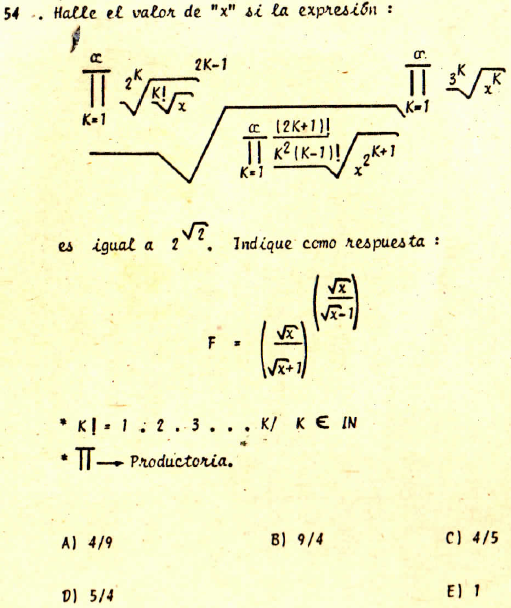
\includegraphics[width=0.95\linewidth]{algebra_pre/Pro_001.png}
}

\LnxSolucion{Solución}{
Sea
$$
	\sqrt[\beta]{\theta}^{\alpha} = 2^{\sqrt{2}}
$$
donde $\alpha, \beta$ y $\theta$ son:
\begin{equation*}
	\scalebox{0.95}{$\displaystyle
			\alpha=\prod_{k= 1}^{\infty} \sqrt[3^k]{x^k}, \quad  \beta = \prod_{k=1}^\infty \left( \sqrt[2^k]{ \sqrt[k!]{x} } \right)^{2k - 1}, \quad \theta = \prod_{k=1}^\infty  \sqrt[\frac{(2k+1)!}{k^2 \cdot (k-1)!} \;\;\; ]{ \displaystyle x^{2^{k+1}}}
		$}
\end{equation*}
Calculamos $\alpha$, [{\small(La demostración de la convergencia queda como ejercicio para el lector)}]
$$
	\alpha=\prod_{k= 1}^{\infty} \sqrt[3^k]{x^k} = (x)^{\sum_{k=1}^{\infty} k\cdot 3^{-k}}
$$
Por la serie geométrica  para \(|u| < 1\),
\begin{equation*}
	\scalebox{0.8}{$\displaystyle
			\sum_{k=1}^\infty k u^k = u \bqty{\dv{u}(\sum_{k=0}^\infty u^k) } = u \bqty{\dv{u}(\frac{1}{1 - u}) }
			= \frac{u}{(1 - u)^2}
		$}
\end{equation*}
$$
	\rightarrow \alpha  =  (x)^{\sum_{k=1}^{\infty} k\cdot 3^{-k}}= (x)^{\frac{ 1/3}{(1-1/3)^2 } } = x^{3/4}
$$

Calculamos $\beta$, [{\small(La demostración de la convergencia queda como ejercicio para el lector)}]
$$
	\beta = \prod_{k=1}^\infty \left( \sqrt[2^k]{ \sqrt[k!]{x} } \right)^{2k - 1} = x ^{ \sum_{k=1}^{\infty} \frac{2k-1}{2^k \cdot k!}}
$$
Calculando  el exponente  $\sum_{k=1}^{\infty} \frac{2k - 1}{2^k \cdot k!}$,

\begin{align*}
	\sum_{k=1}^{\infty} \frac{2k - 1}{2^k \cdot k!}
	 & = \sum_{k=1}^\infty \frac{1}{2^{k-1} \cdot (k-1)!} - \sum_{k=1}^\infty \frac{1}{2^k \cdot k!} \\
	 & = \sum_{k=0}^\infty \frac{1}{2^k \cdot k!} - \sum_{k=1}^\infty \frac{1}{2^k \cdot k!}  = 1
\end{align*}
$$
	\Rightarrow \beta =x^{1}=x
$$
Calculamos $\theta$, [{\small(La demostración de la convergencia queda como ejercicio para el lector)}]
\[
	\theta = \prod_{k=1}^\infty  \sqrt[\frac{(2k+1)!}{k^2 \cdot (k-1)!} \;\;\; ]{ \displaystyle x^{2^{k+1}}}  = (x)^{\sum_{k=1}^\infty \frac{2^{k+1}\cdot k^2 \cdot (k-1)!}{ (2k+1)!}}
\]
Calculando  el exponente  $ \sum_{k=1}^\infty \frac{2^{k+1}\cdot k^2 \cdot (k-1)!}{ (2k+1)!}$,
\begin{align*}
	\sum_{k=1}^\infty \frac{2^{k+1}\cdot k  \cdot (k )!}{ (2k+1)!} & =\frac{1}{2}\bqty{   \sum_{k=1}^\infty \frac{2^{k}  \cdot (k-1 )!}{ (2k-1)!}- \frac{2^{k+1}\cdot   (k )!}{ (2k+1)!}}                      \\
	                                                               & =\frac{1}{2}\pqty{2+\sum_{k=1}^\infty \frac{2^{k+1}\cdot   (k )!}{ (2k+1)!} - \sum_{k=1}^\infty \frac{2^{k+1}\cdot   (k )!}{ (2k+1)!} }=1
\end{align*}
$$
	\rightarrow \theta = x ^1 = x
$$
Entonces, reemplazando $\alpha, \beta $ y $\theta$:
$$
	\sqrt[\beta]{\theta}^{\alpha} =\sqrt[x]{x}^{x^{3/4}} = x^{x^{-1/4}} =2^{\sqrt{2}}
$$
Elevamos a $(-1/4)$
$$
	\pqty{x^{-1/4}}^{\pqty{ x^{-1/4}}} = \pqty{2^{\sqrt{2}} }^{-1/4}= \pqty{\frac{1}{2}}^{\frac{\sqrt{2}}{4}}= \pqty{\frac{1}{\sqrt{2}}}^{\pqty{\frac{1}{\sqrt{2}}}}
$$
$$
	x^{-1/4} = \frac{1}{\sqrt{2}} \Rightarrow x^{1/4} = \sqrt{2} \Rightarrow x = (\sqrt{2})^4 = 4
$$

Finalmente, reemplazamos $x$ en $F$,
}

\begin{LnxRptaBox}
	\[
		F= \pqty{\frac{\sqrt{x}}{\sqrt{x}+1}}^{\pqty{\frac{\sqrt{x}}{\sqrt{x}-1}}} = \pqty{\frac{2}{3}}^{\frac{2}{1}}= \frac{4}{9}
	\]
\end{LnxRptaBox}
  
	
	%%corregir el problema 2
\end{document}